\documentclass[12pt,a4paper]{article}
\usepackage[utf8]{inputenc}
\usepackage{graphicx}
\usepackage{geometry}
\usepackage{fancyhdr}
\usepackage{listings}
\usepackage{xcolor}
\usepackage{float}
\usepackage[colorlinks=false,hidelinks]{hyperref}

\geometry{margin=1in}
\pagestyle{fancy}
\fancyhf{}
\rhead{FIT5032 - Assessed Lab 11}
\cfoot{\thepage}

% Code listing style
\lstset{
    basicstyle=\ttfamily\small,
    breaklines=true,
    frame=single,
    numbers=left,
    numberstyle=\tiny,
    commentstyle=\color{green!50!black},
    keywordstyle=\color{blue},
    stringstyle=\color{red}
}

\title{FIT5032 Assessed Lab 11\\
Deployment using Cloudflare Pages}
\author{Student Name: [Du Daoan]\\
Student ID: [35523166]}
\date{}

\begin{document}

\maketitle

\tableofcontents
\newpage

\section{EFOLIO TASK 11.1 (PASS AND CREDIT LEVEL)}

\subsection{Project Deployment Link}

\textbf{Deployed Project URL:} \texttt{https://your-project-name.pages.dev}

\subsection{Cloudflare Deployment Success Screenshot}

% Screenshot showing successful Cloudflare Pages deployment
\begin{figure}[H]
\centering
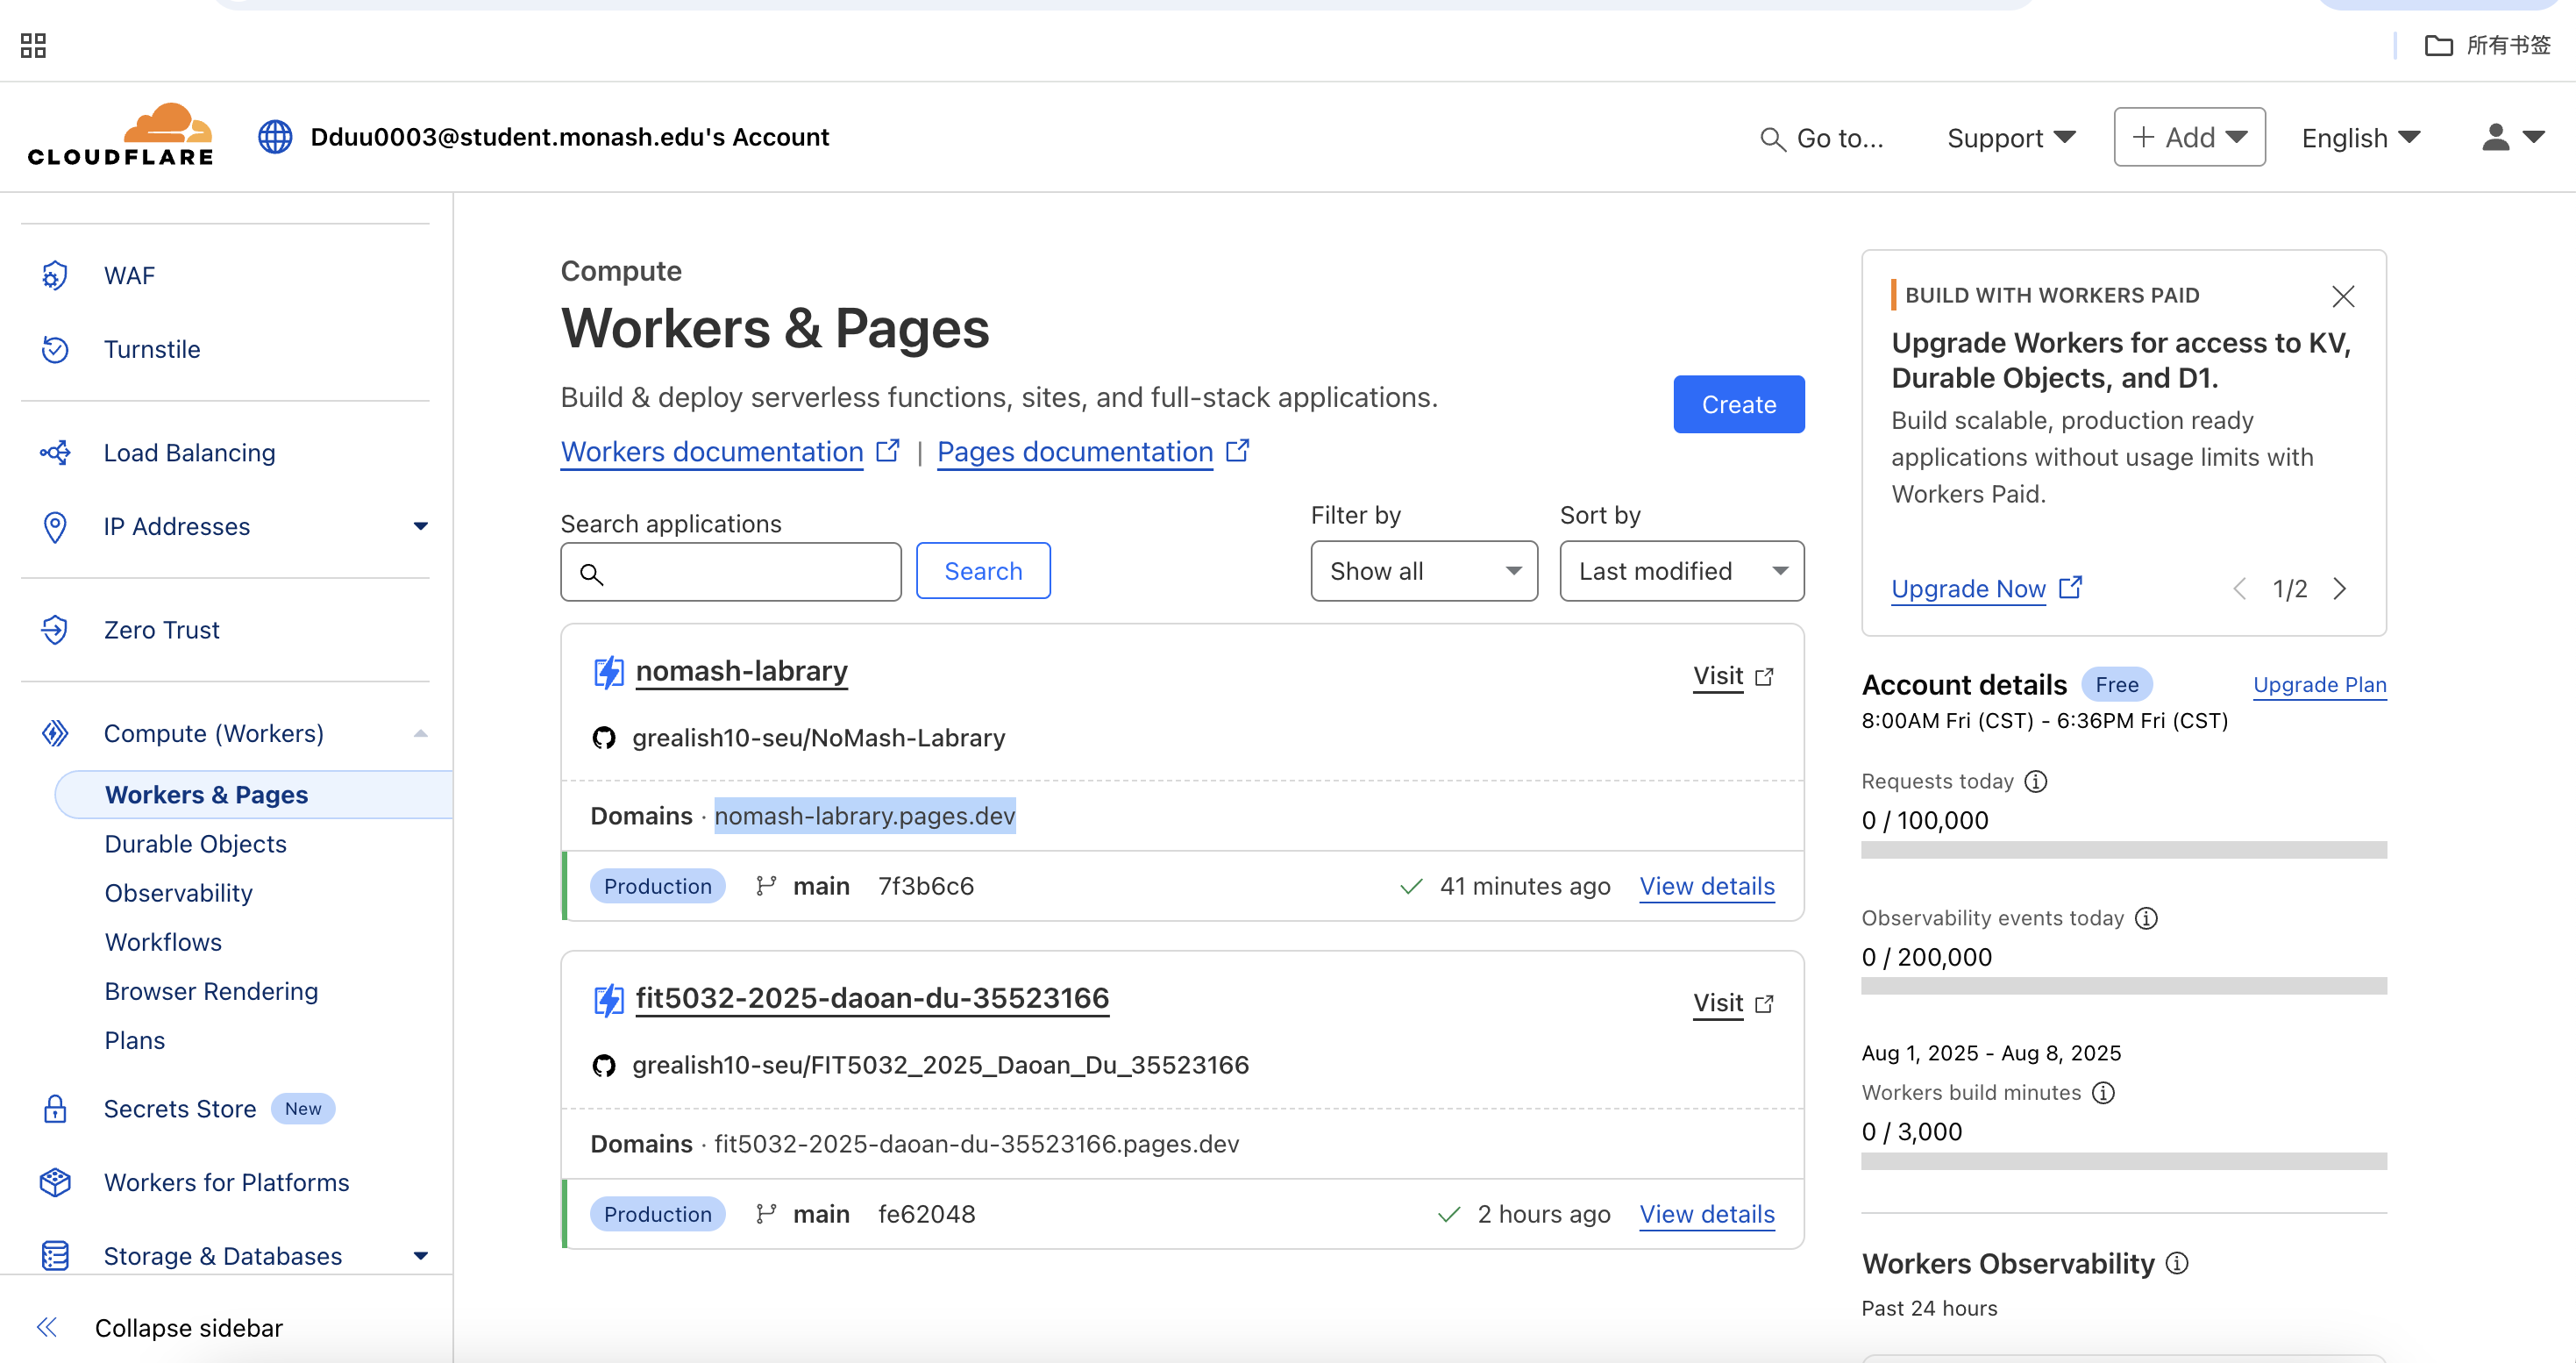
\includegraphics[width=0.9\textwidth]{cloudflare_deployment_success.png}
\caption{Cloudflare Pages deployment success page showing project name, successful deployment status, and generated domain}
\end{figure}

This screenshot demonstrates:
\begin{itemize}
\item Successful deployment to Cloudflare Pages
\item Generated domain URL for the project
\item Deployment timestamp and build information
\item Cloudflare interface elements confirming the deployment
\end{itemize}

\subsection{Project Homepage Screenshot}

% Screenshot showing the deployed project homepage
\begin{figure}[H]
\centering
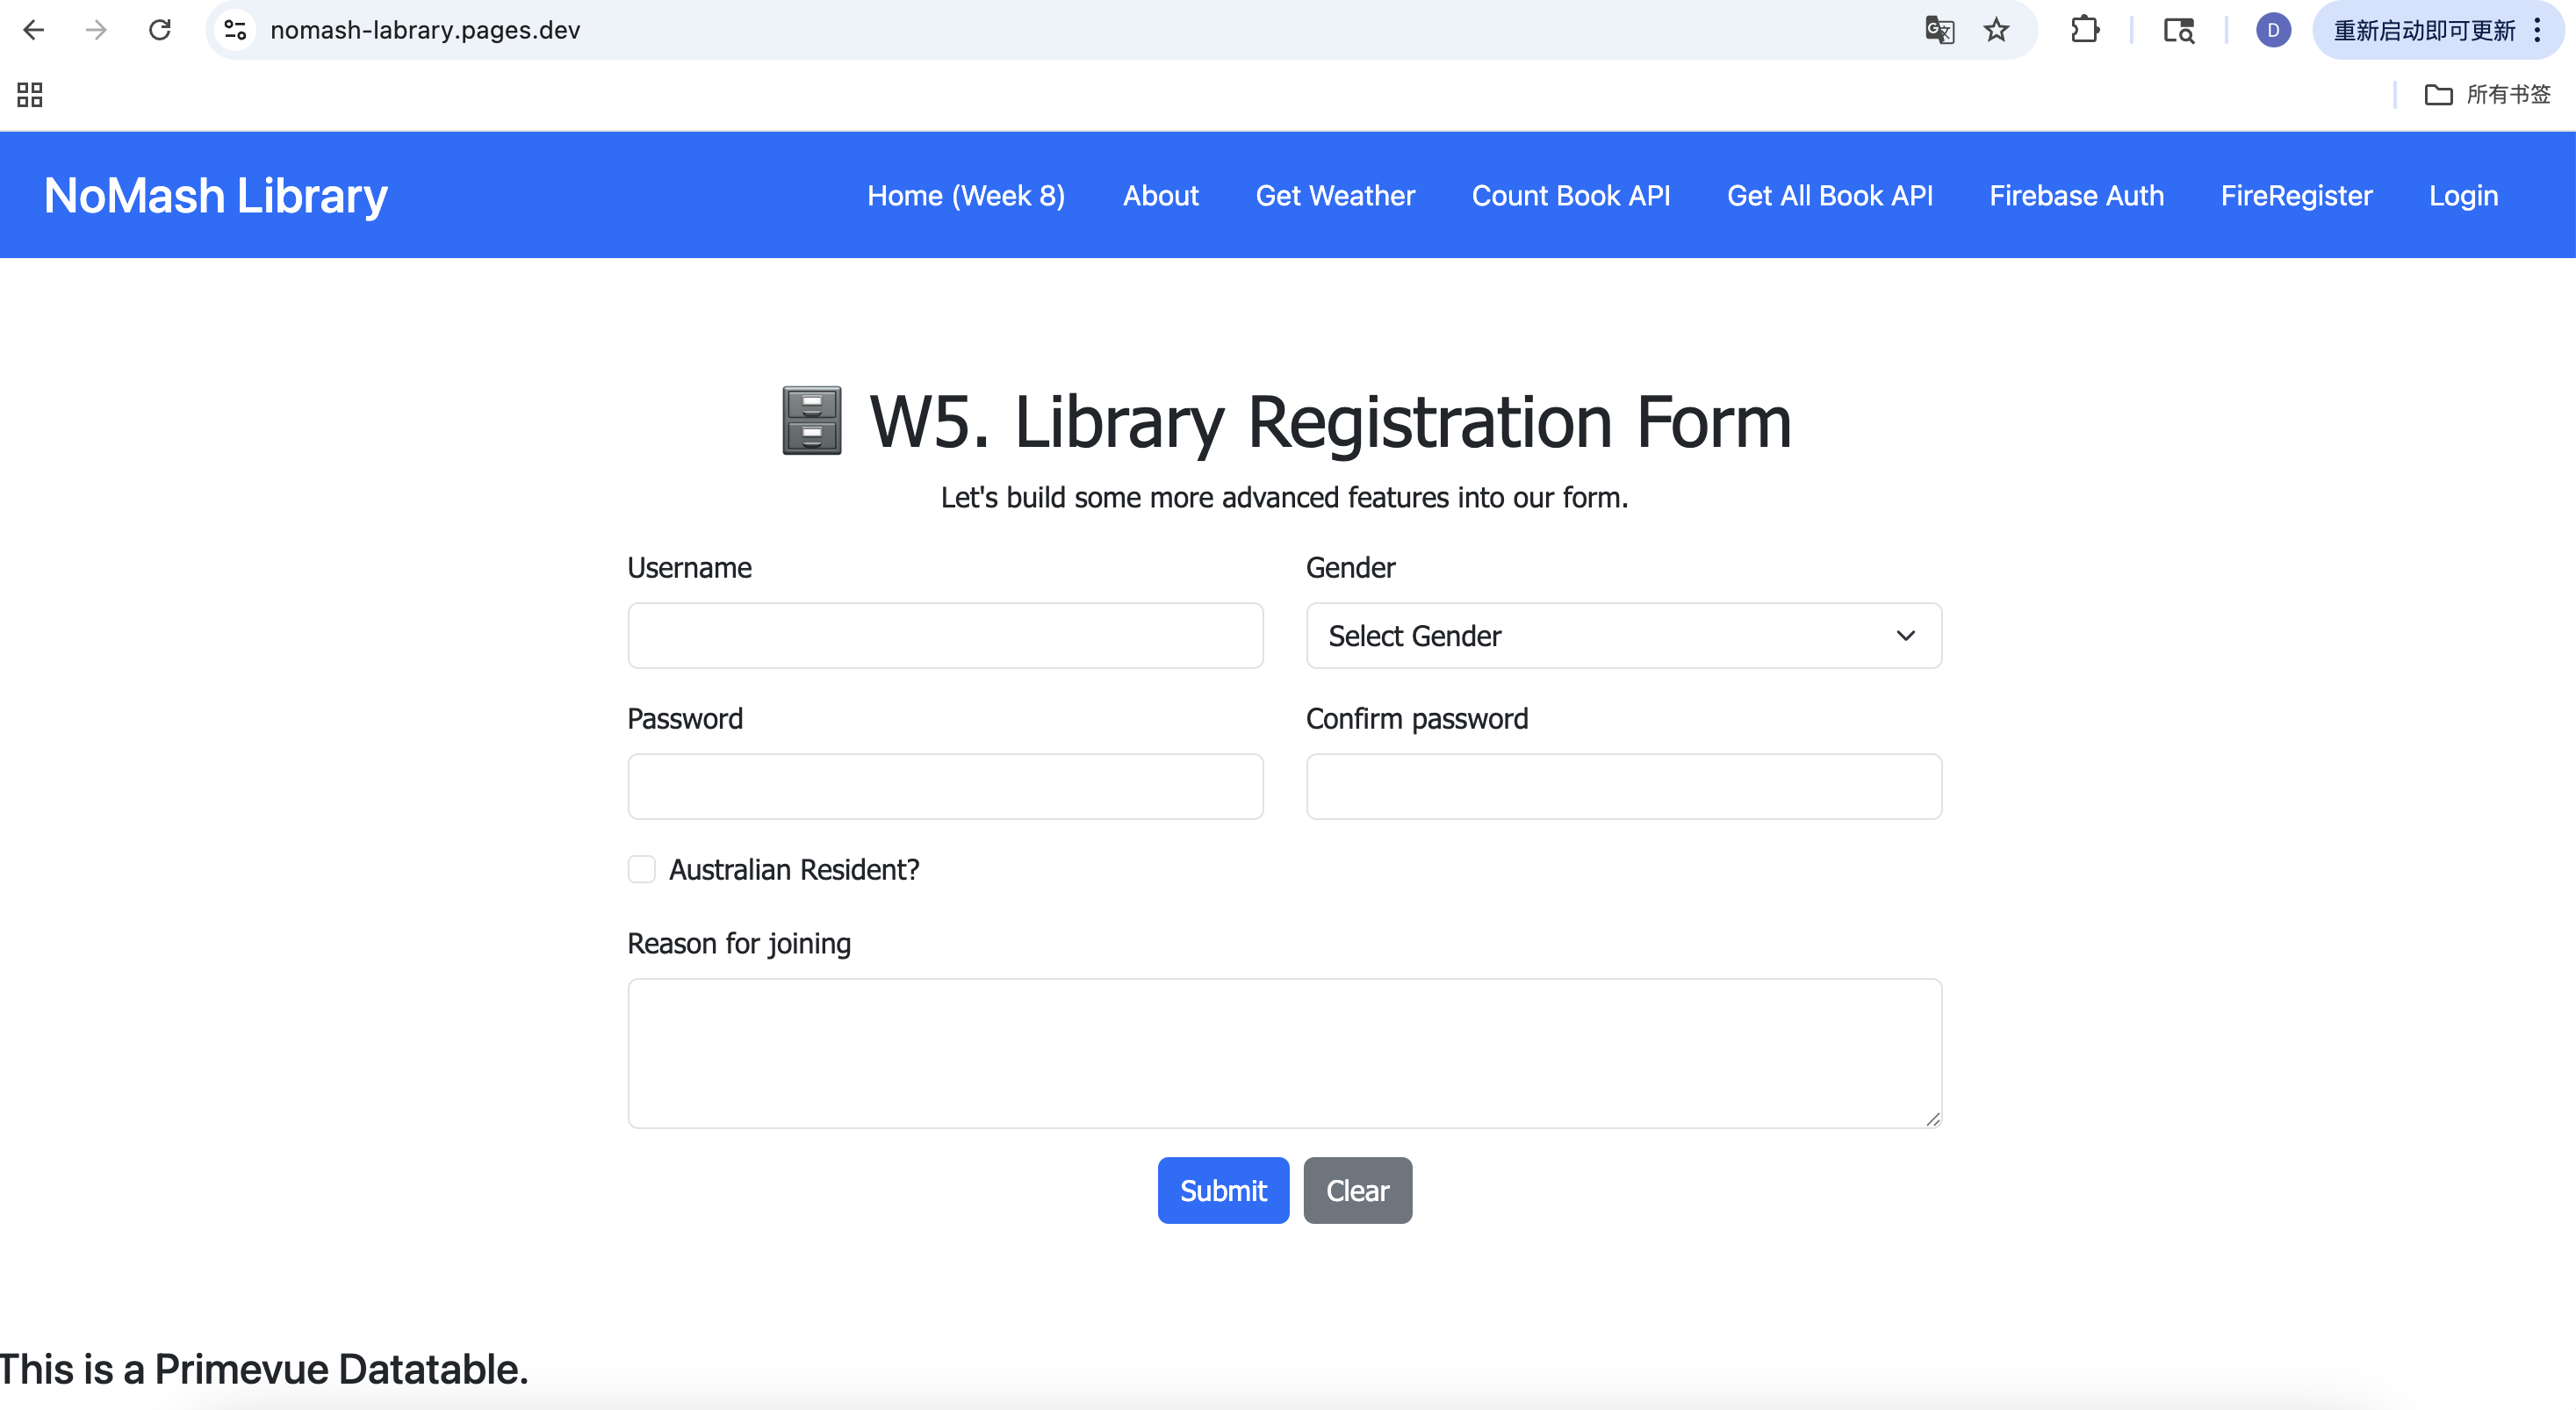
\includegraphics[width=0.9\textwidth]{deployed_homepage.png}
\caption{Deployed NoMash Library homepage showing registration form and navigation}
\end{figure}

The homepage successfully displays:
\begin{itemize}
\item Library registration form
\item Navigation menu with all implemented features
\item Responsive design elements
\item Functional user interface components
\end{itemize}

\newpage

\section{EFOLIO TASK 11.2 (DISTINCTION AND HIGH DISTINCTION LEVEL)}

\subsection{WeatherCheck Page Functionality}

\subsubsection{Weather Page Address Bar Screenshot}

% Screenshot showing WeatherCheck page with visible address bar
\begin{figure}[H]
\centering
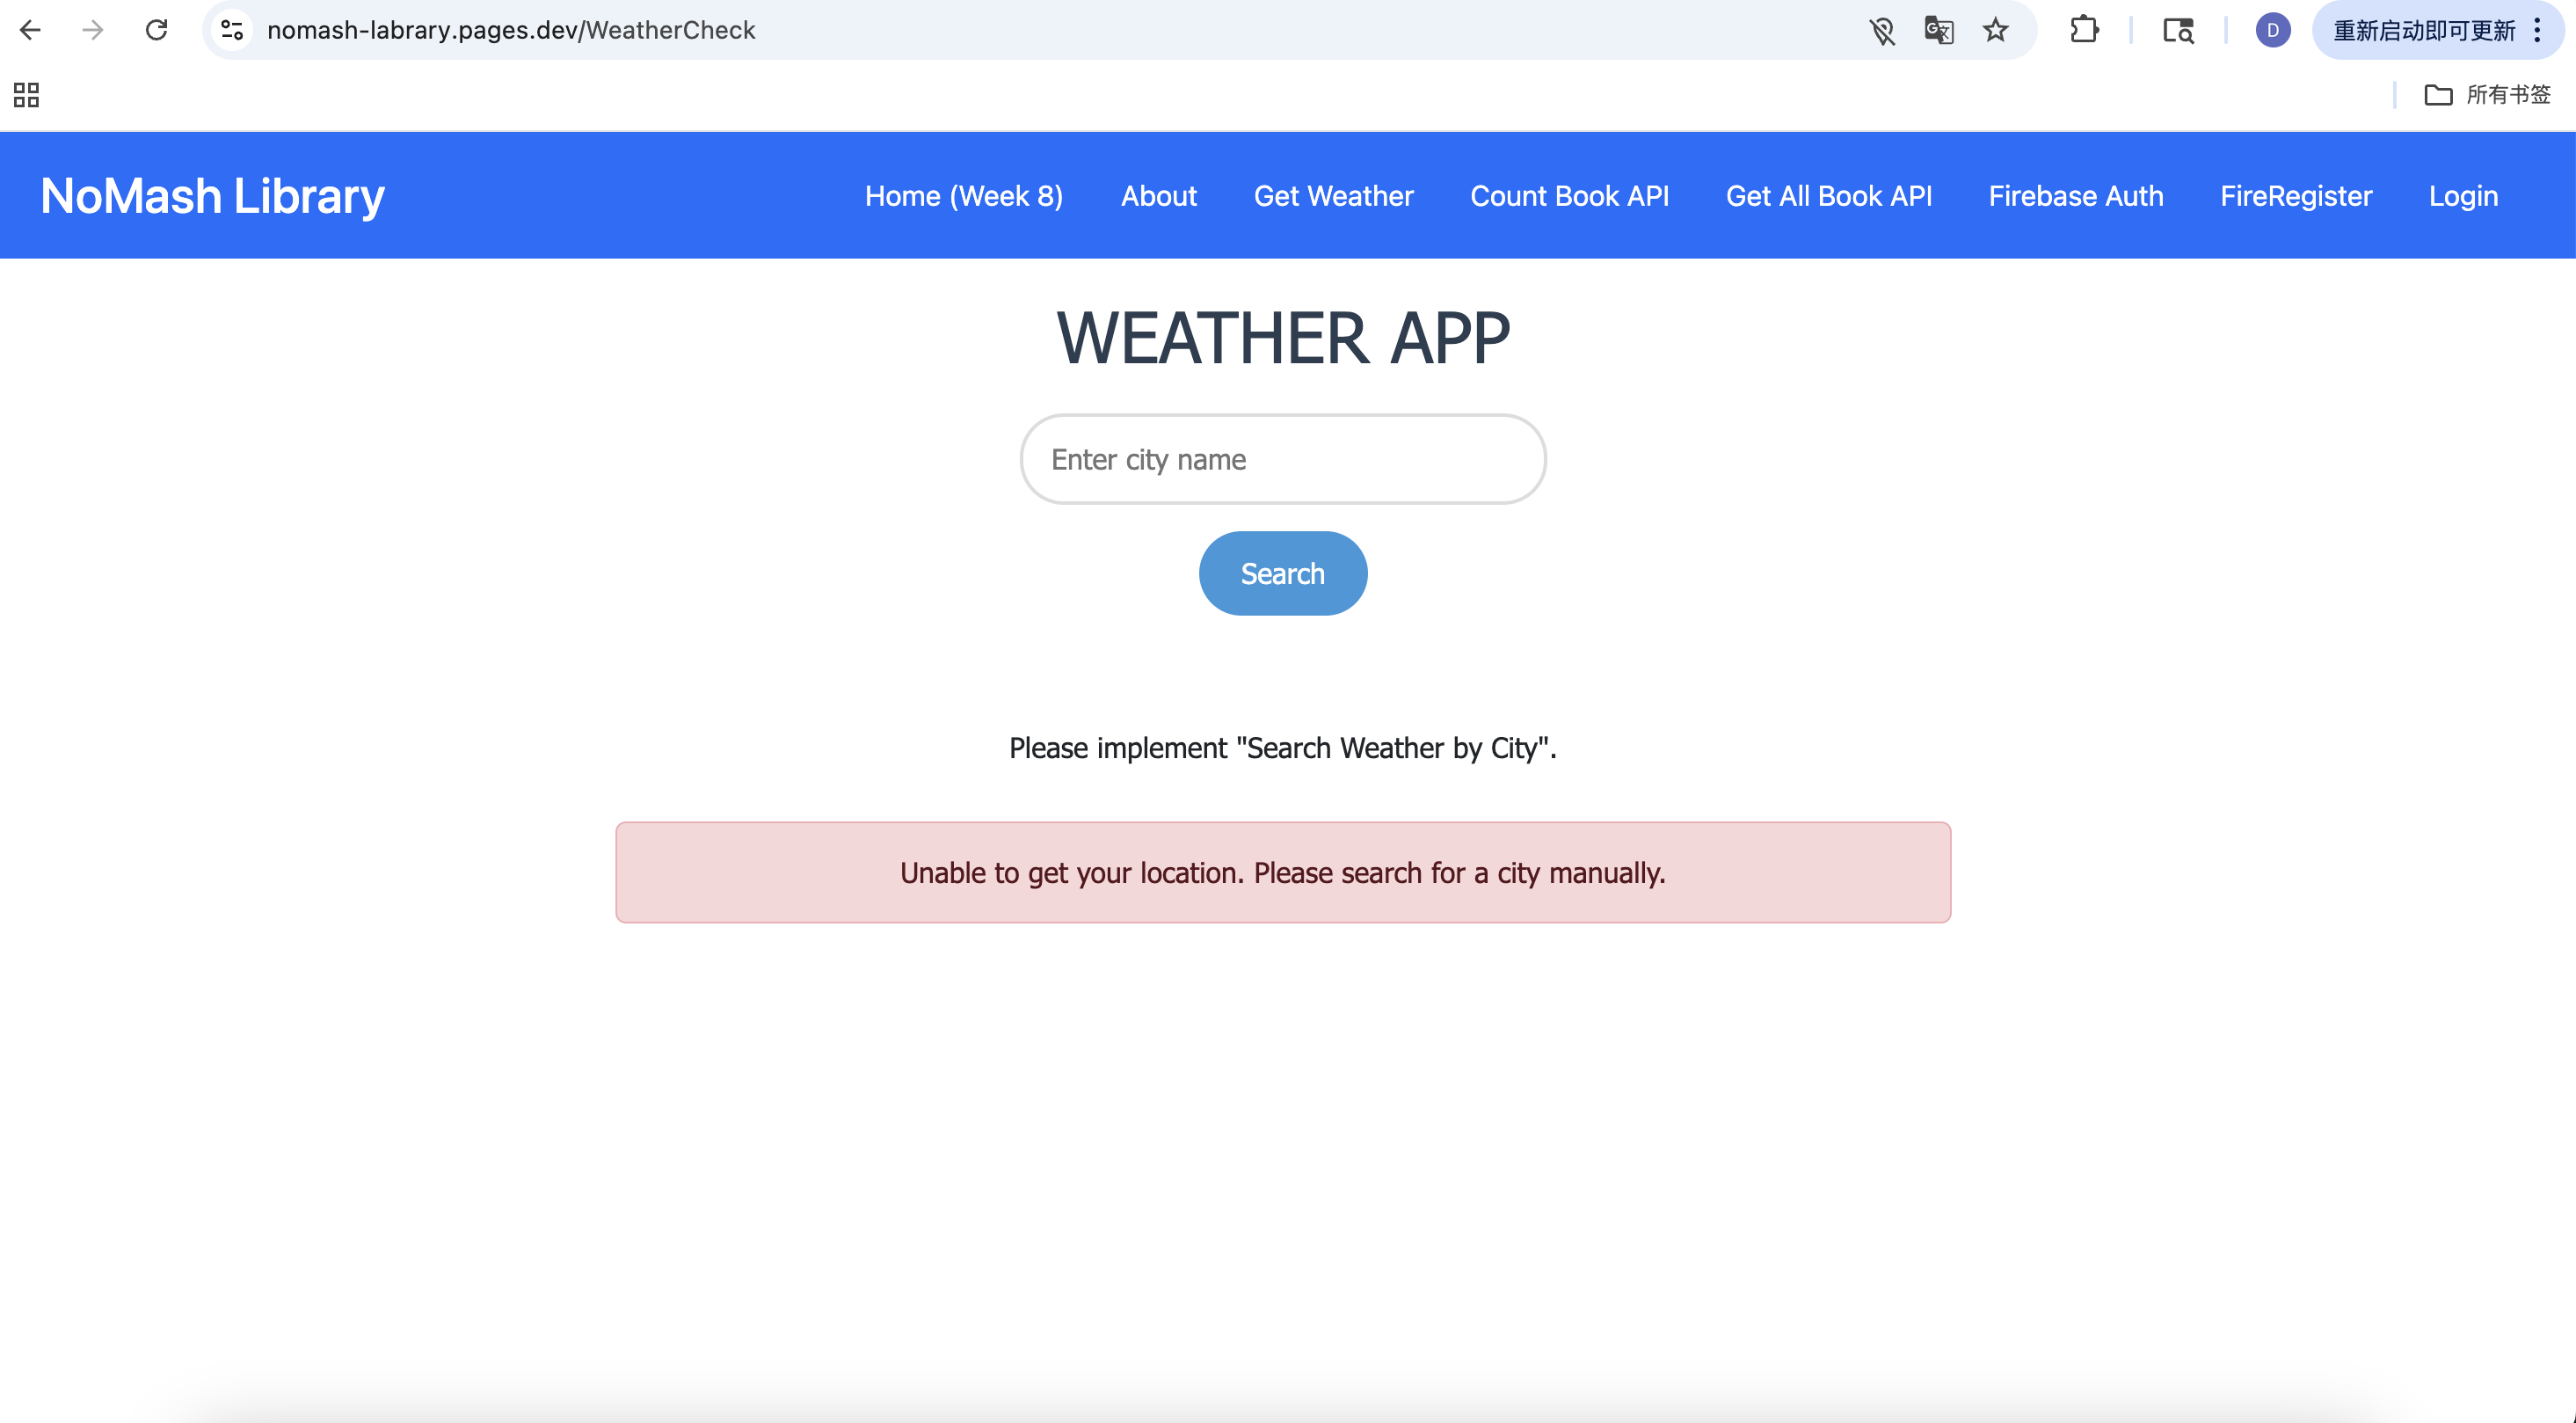
\includegraphics[width=0.9\textwidth]{weather_page_addressbar.png}
\caption{WeatherCheck page with address bar showing https://your-domain.pages.dev/WeatherCheck}
\end{figure}

This screenshot proves:
\begin{itemize}
\item Correct URL routing to /WeatherCheck page
\item Page loads successfully in production environment
\item Address bar clearly visible with full domain path
\end{itemize}

\subsubsection{Weather Functionality Working Screenshot}

% Screenshot showing weather data and search functionality
\begin{figure}[H]
\centering
% 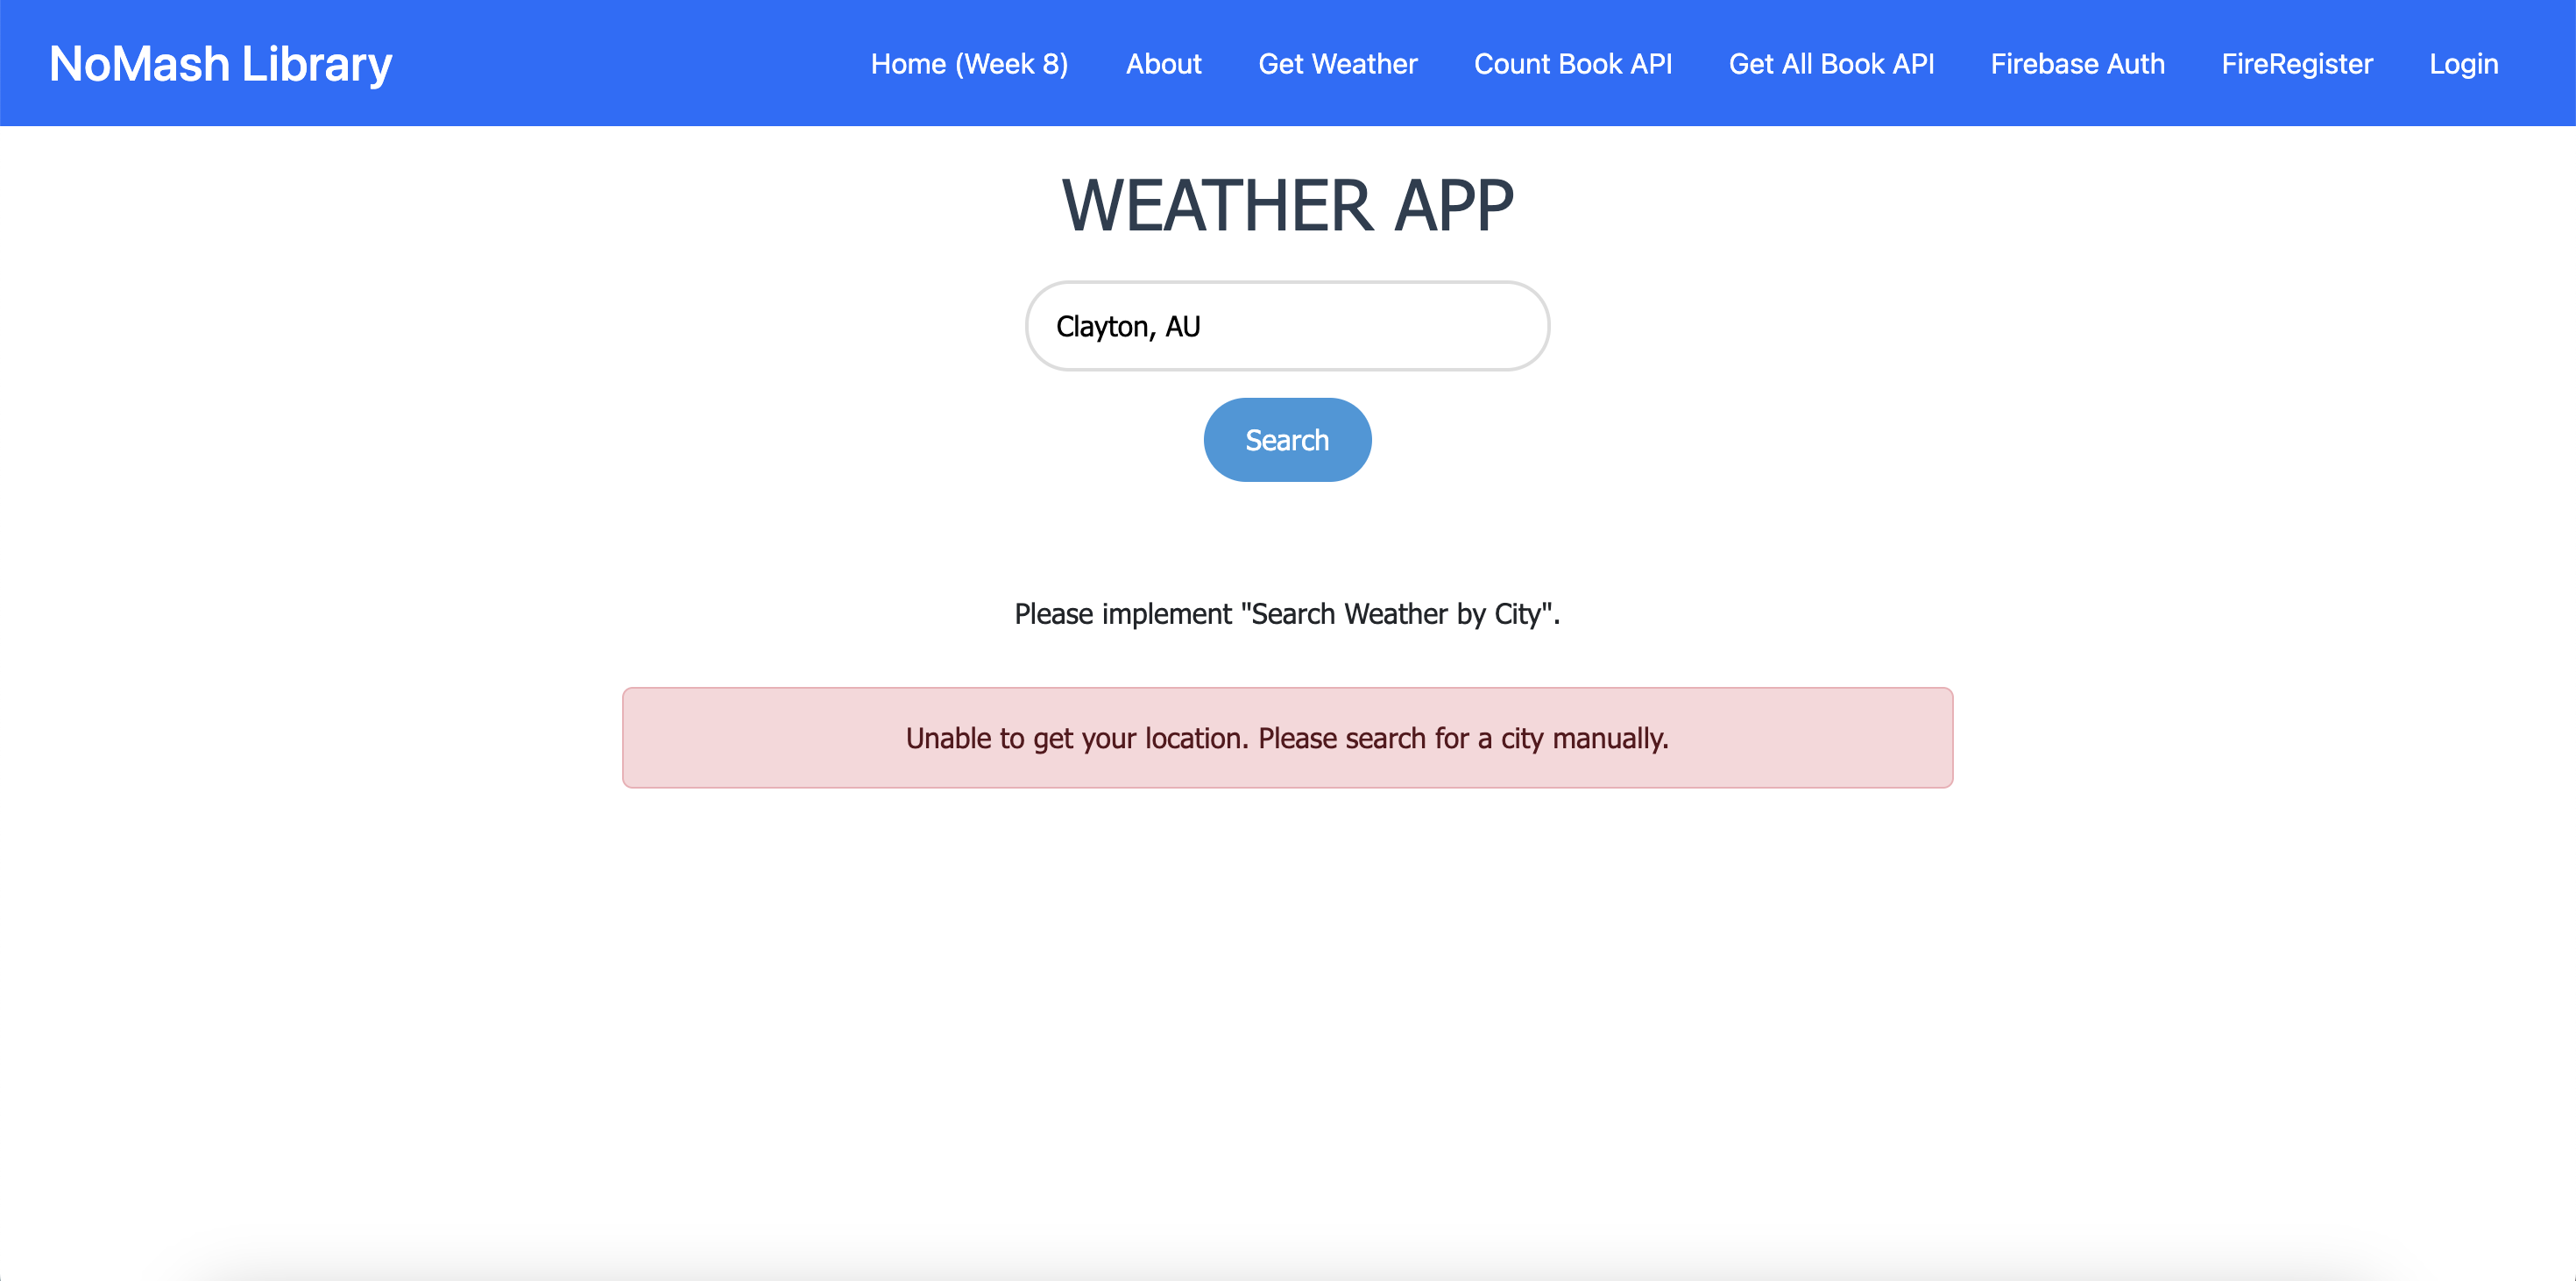
\includegraphics[width=0.9\textwidth]{weather_functionality_working.png}
\caption{Weather application showing search functionality and weather data display}
\end{figure}

The weather functionality demonstrates:
\begin{itemize}
\item Search input field accepting city names
\item Search button functionality
\item Weather data display (temperature, conditions, details)
\item Proper integration with OpenWeatherMap API
\end{itemize}

\subsubsection{Weather Search Results Screenshot}

% Screenshot showing successful weather search for Clayton
\begin{figure}[H]
\centering
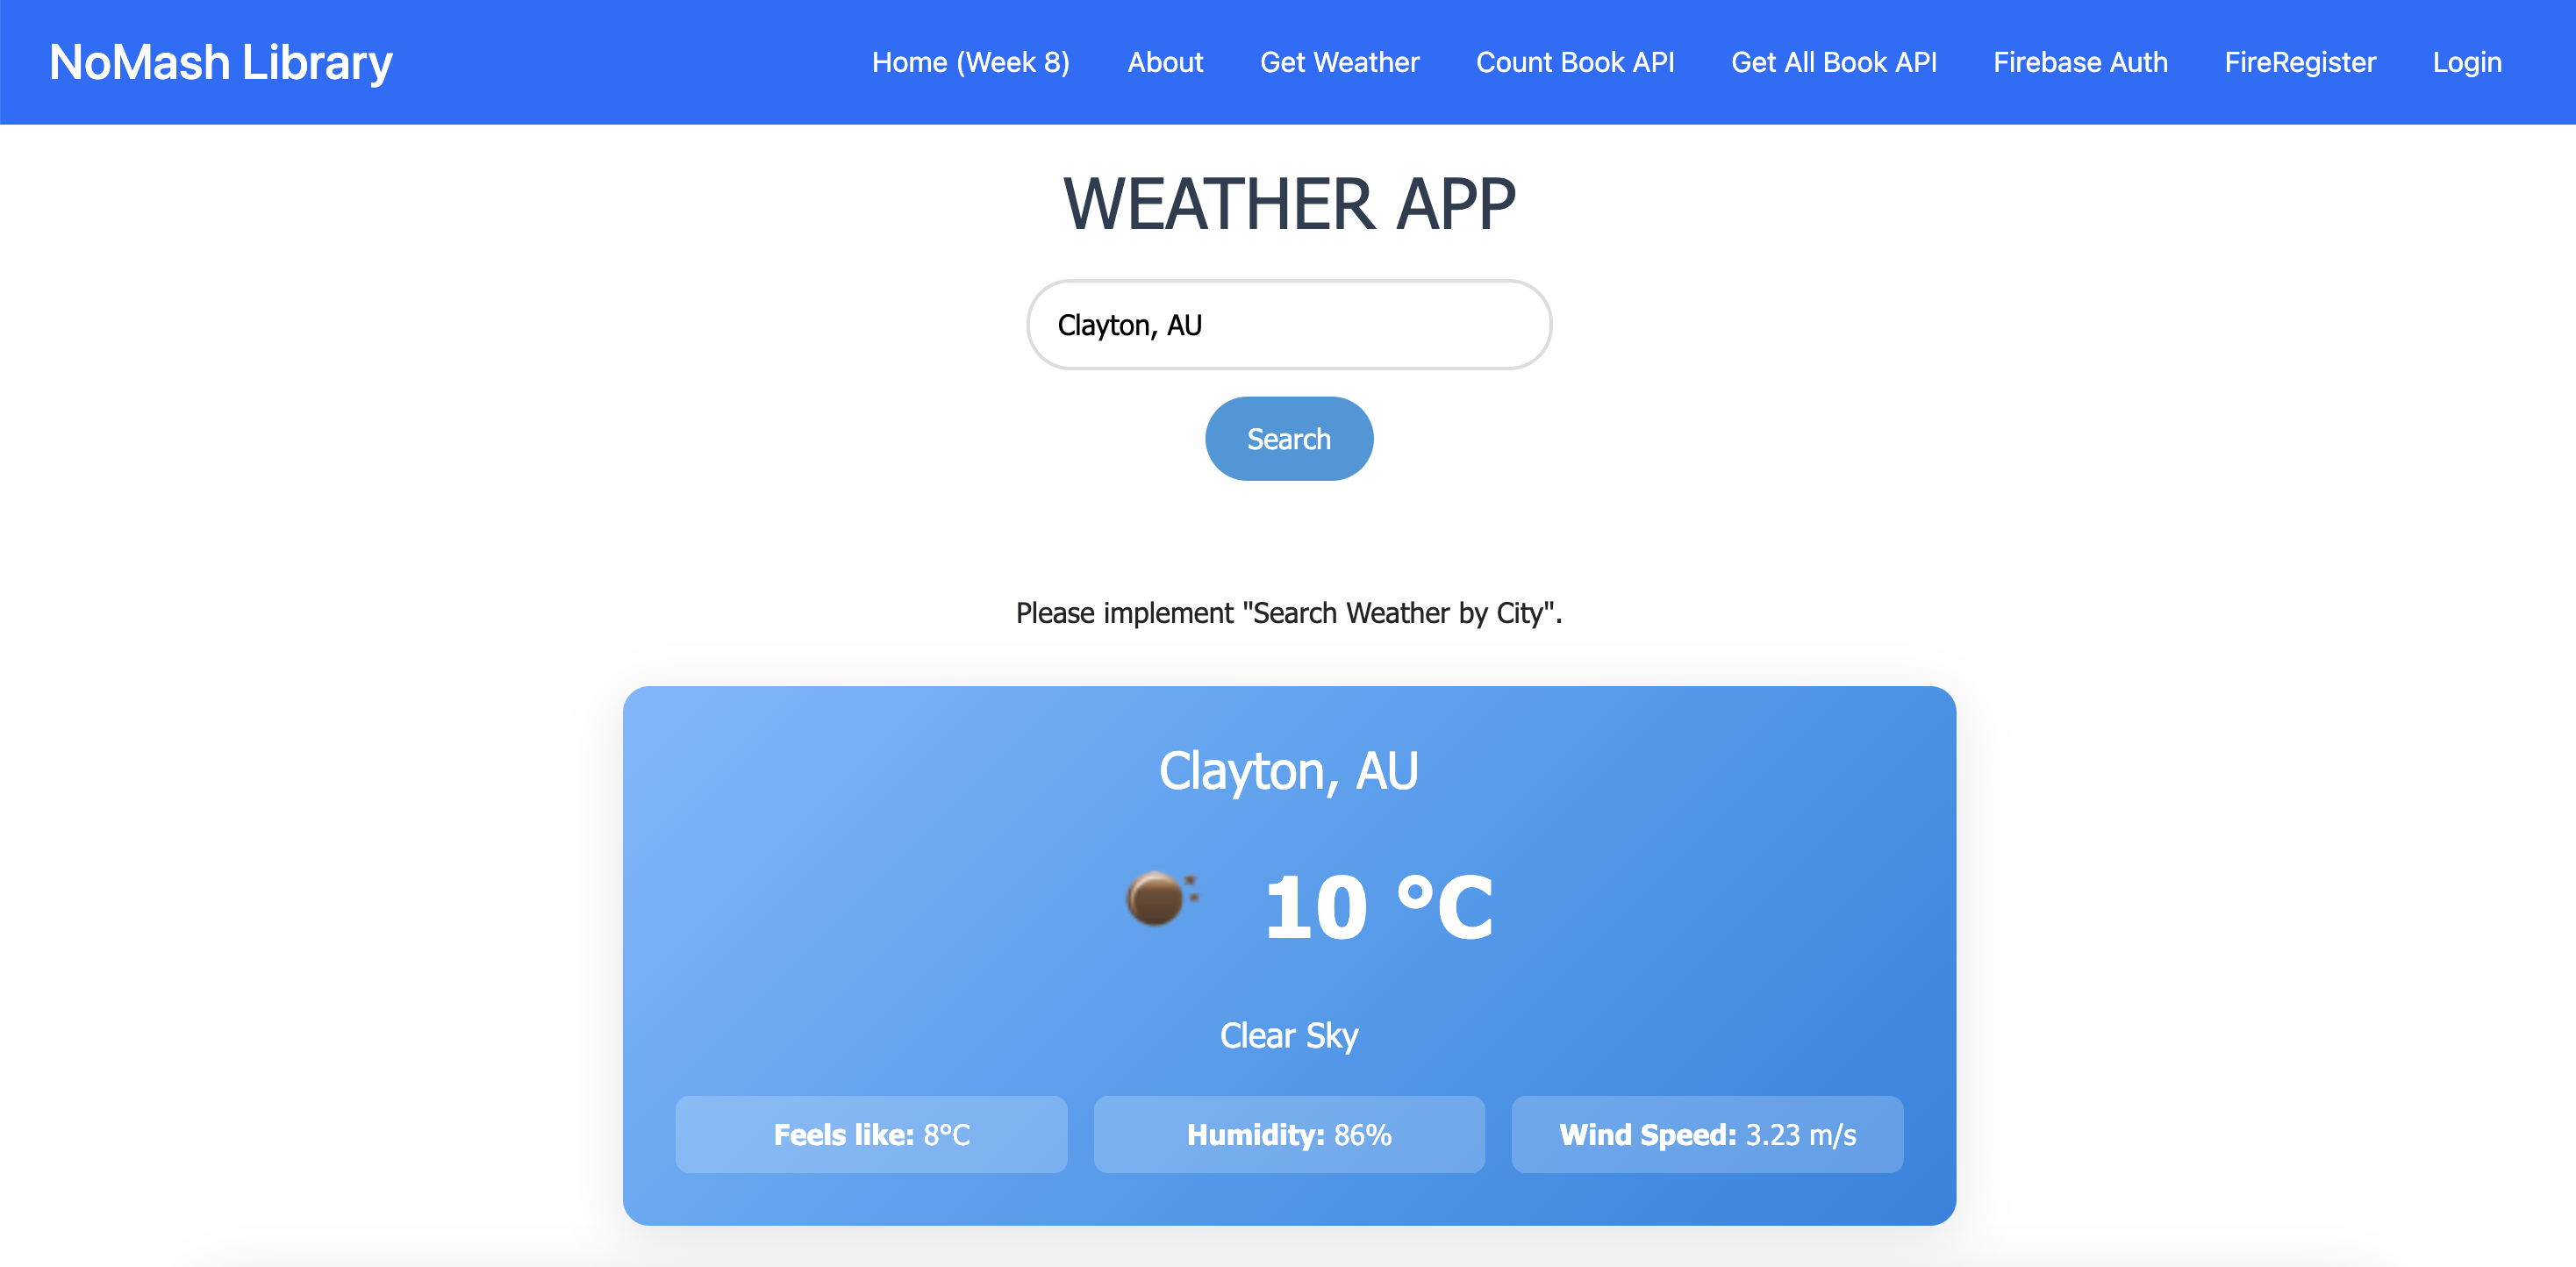
\includegraphics[width=0.9\textwidth]{clayton_weather_search.png}
\caption{Successful weather search for Clayton, AU showing temperature and weather conditions}
\end{figure}

Successful search results show:
\begin{itemize}
\item City name: Clayton, AU
\item Current temperature in Celsius
\item Weather icon and description
\item Additional details (feels like, humidity, wind speed)
\end{itemize}

\newpage

\section{Technical Implementation Summary}

\subsection{Deployment Configuration}

The project was successfully deployed using the following configuration:

\begin{lstlisting}
Framework Preset: Vue
Build Command: npm run build
Build Output Directory: dist
Production Branch: main
Repository: grealish10-seu/NoMash-Labrary
\end{lstlisting}

\subsection{Key Features Deployed}

\begin{itemize}
\item Vue.js single-page application
\item Vue Router for navigation
\item Firebase Authentication integration
\item Firestore database connectivity
\item External API integration (OpenWeatherMap)
\item Local API services (CountBookAPI, GetAllBookAPI)
\item Responsive design with Bootstrap
\end{itemize}

\subsection{Post-Deployment Verification}

All major functionalities verified in production:
\begin{itemize}
\item Homepage and navigation working
\item User authentication system functional
\item Weather API integration operational
\item Database operations accessible
\item All routes properly configured
\end{itemize}

\newpage

\end{document} 